\documentclass{article}
\usepackage{graphicx}
\usepackage{float}

\usepackage{caption}
\usepackage{subcaption}

\usepackage[utf8]{inputenc}

\begin{document}

\author{Antonella Dellanzo}
\title{Guía 1 - Introducción al procesamiento digital de imágenes}
\date{}
\maketitle

\section*{Ejercicio 1 - a}
Los archivos correspondientes a cada ejercicio son:
\begin{itemize}
\item \textbf{Suma: } sumaDeImagenes.m
\item \textbf{Resta: } restaDeImagenes.m
\item \textbf{Producto: } productoDeImagenes.m
\end{itemize}
Cada uno tomando como input las dos imágenes a ser sumadas. Si las imágenes no son del mismo tamaño, se produce un error. Este inciso se puede probar con una imagen de lena y la de fingerprints.

\section*{Ejercicio 1 - b}
El archivo correspondiente es \textit{productoImagenEscalar.m} y toma como parámetros de entrada una imagen y un valor númerico correspondiente al escalar deseado. Este inciso se puede probar con una imagen de lena y la de fingerprints.

\section*{Ejercicio 1 - c}
El archivo correspondiente es \textit{compresionRangoDinamico.m} y toma como parámetro de entrada una imagen. Este ejercicio se puede probar con la imagen llamada \textit{oscura.png}.

\section*{Ejercicio 2}
El archivo correspondiente es \textit{negativoDeImagen.m} y toma como parámetro de entrada una imagen. Este ejercicio se puede probar con la imagen de lena.

\section*{Ejercicio 3}
El archivo correspondiente es \textit{umbral.m} y toma como parámetros de entrada una imagen y un valor númerico que es el umbral correspondiente. Éste último valor debe ser menor a 256 (valor de gris de 8 bits con el que se trabaja). En caso contrario se producirá un error. El output es una imagen lógica que resuelve la umbralización de dicha imagen con dicho umbral. Este ejercicio se puede probar con la imagen de lena.

\section*{Ejercicio 4}
Para este ejercicio se encuentran 2 archivos adjuntos, cuyo parámetro de entrada es una imagen:
\begin{itemize}
\item \textbf{separarEnOchoPlanosDeBits.m: }Genera el fraccionamiento en 8 planos de bits y los muestra todos en una misma figura utilizando la función \textit{subplot}.
\item \textbf{separarEnOchoPlanosDeBitsMostrandoEnFiguras.m: }Genera el fraccionamiento en 8 planos de bits y muestra cada imagen en una figura distinta (cada una posee el título correspondiente al plano de bit).
\end{itemize}

A continuación presento un ejemplo de lo producido al ejecutar la primera función:

\begin{figure}[H]
   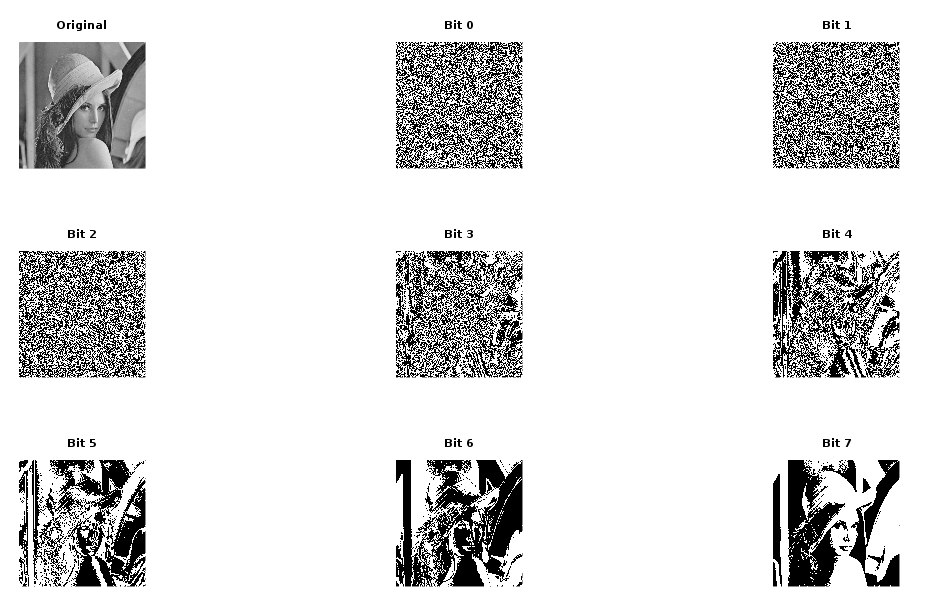
\includegraphics[width=0.9\textwidth]{planobitslena.png} % first figure itself
    \caption{Fraccionamiento en 8 planos de bit de imagen de Lena}
\end{figure}

\section*{Ejercicio 5}
Para este ejercicio se encuentran 2 archivos adjuntos, cuyo parámetro de entrada es una imagen:
\begin{itemize}
\item \textbf{histograma.m: }Genera el histograma no normalizado de una imagen, mostrando el gráfico de barras del mismo y devolviendo como output dicho vector.
\item \textbf{histogramaNormalizado.m: } Genera el histograma normalizado de una imagen, mostrando el gráfico de barras del mismo y devolviendo como output dicho vector.
\end{itemize}

A continuación presento ejemplos al ejecutar dichas funciones:

\begin{figure}[H]
    \begin{subfigure}{0.5\textwidth}
        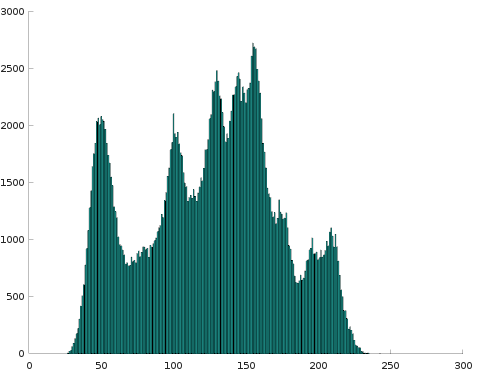
\includegraphics[width=0.9\textwidth]{histoLena.png} % first figure itself
    \subcaption{Histograma de imagen de Lena}
    \end{subfigure}\hfill
    \begin{subfigure}{0.5\textwidth}
        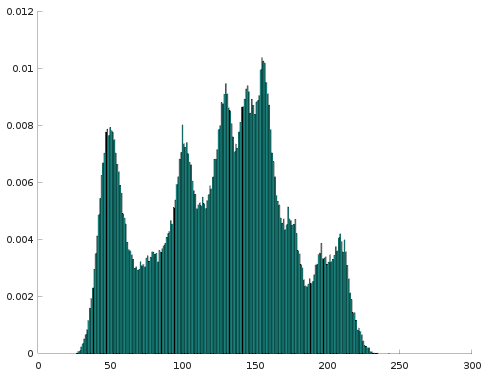
\includegraphics[width=0.9\textwidth]{histoNormalizadoLena.png} % second figure itself
    \subcaption{Histograma noramlizado de imagen de Lena ecualizada}
    \end{subfigure}
\end{figure}

\section*{Ejercicio 7}
El archivo correspondiente es \textit{ecualizacion.m} y toma como parámetro de entrada una imagen. El output del programa es la imagen ecualizada. 

Al ejecutar el archivo con la imagen de Lena, se pueden observar los siguientes resultados:
\begin{figure}[H]
    \begin{subfigure}{0.5\textwidth}
        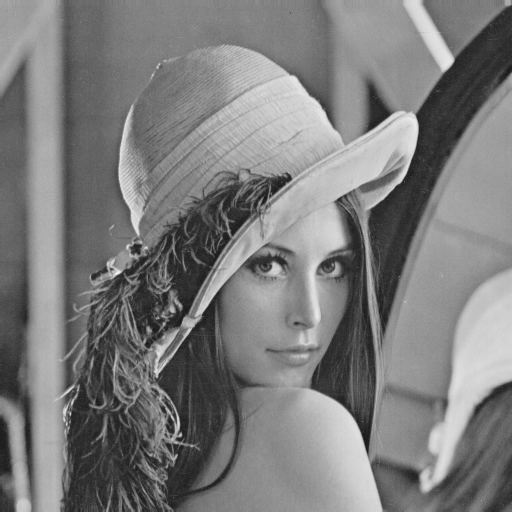
\includegraphics[width=0.9\textwidth]{lena.png} % first figure itself
    \subcaption{Imagen de Lena original}
    \end{subfigure}\hfill
    \begin{subfigure}{0.5\textwidth}
        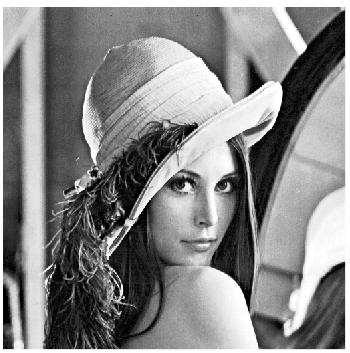
\includegraphics[width=0.9\textwidth]{lenaEq.png} % second figure itself
    \subcaption{Imagen de Lena ecualizada}
    \end{subfigure}
\end{figure}

\begin{figure}[H]
    \begin{subfigure}{0.5\textwidth}
        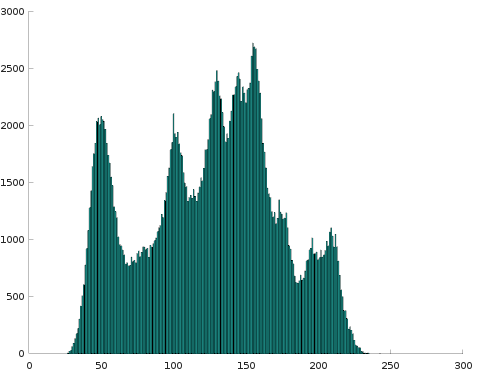
\includegraphics[width=0.9\textwidth]{histoLena.png} % first figure itself
    \subcaption{Histograma de imagen de Lena original}
    \end{subfigure}\hfill
    \begin{subfigure}{0.5\textwidth}
        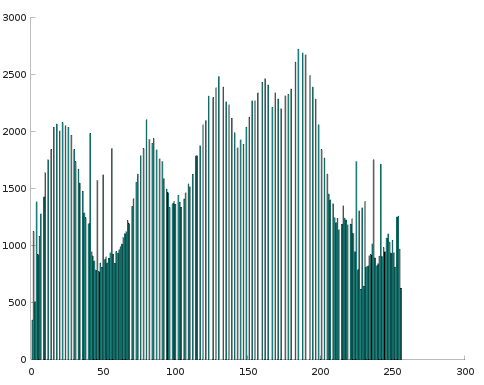
\includegraphics[width=0.9\textwidth]{histoLenaEq.png} % second figure itself
    \subcaption{Histograma de imagen de Lena ecualizada}
    \end{subfigure}
\end{figure}

\begin{figure}[H]
    \begin{subfigure}{0.5\textwidth}
        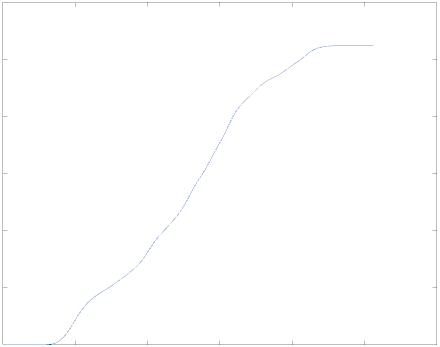
\includegraphics[width=0.9\textwidth]{histoAcumLena.png} % first figure itself
    \subcaption{Histograma acumulado de imagen de Lena original}
    \end{subfigure}\hfill
    \begin{subfigure}{0.5\textwidth}
        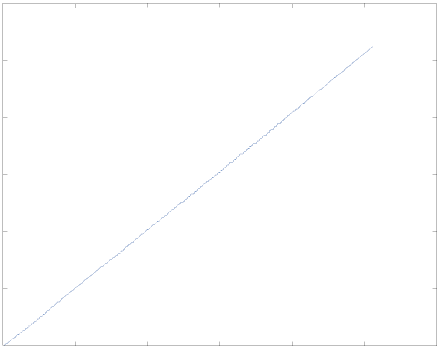
\includegraphics[width=0.9\textwidth]{histoAcumLenaEq.png} % second figure itself
    \subcaption{Histograma acumulado de imagen de Lena ecualizada}
    \end{subfigure}
\end{figure}

\section*{Ejercicio 8}
\begin{figure}[H]
    \begin{subfigure}{0.5\textwidth}
        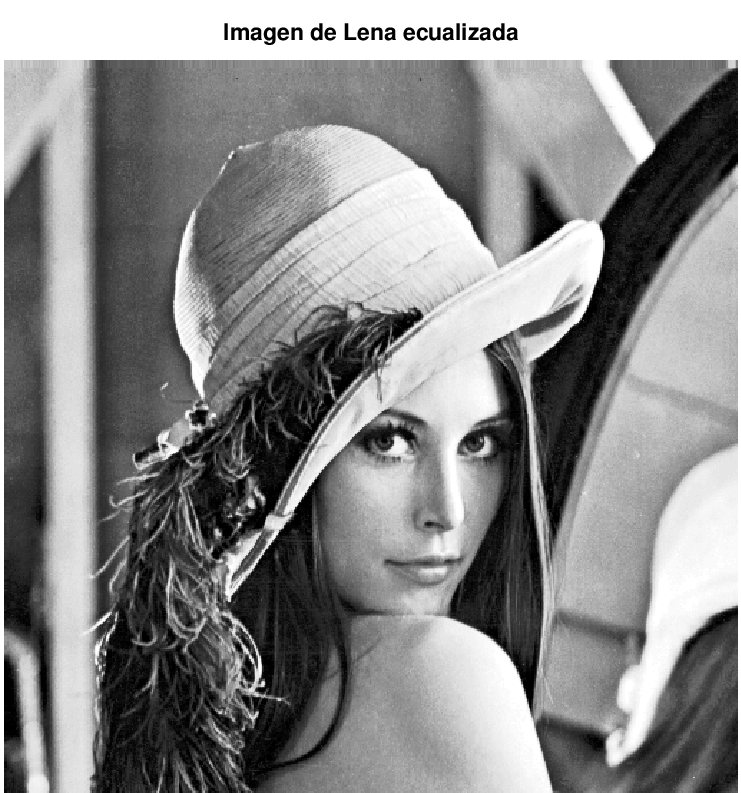
\includegraphics[width=0.9\textwidth]{lenaEcualizada.png} % first figure itself
    \subcaption{Imagen de Lena ecualizada 1 vez}
    \end{subfigure}\hfill
    \begin{subfigure}{0.5\textwidth}
        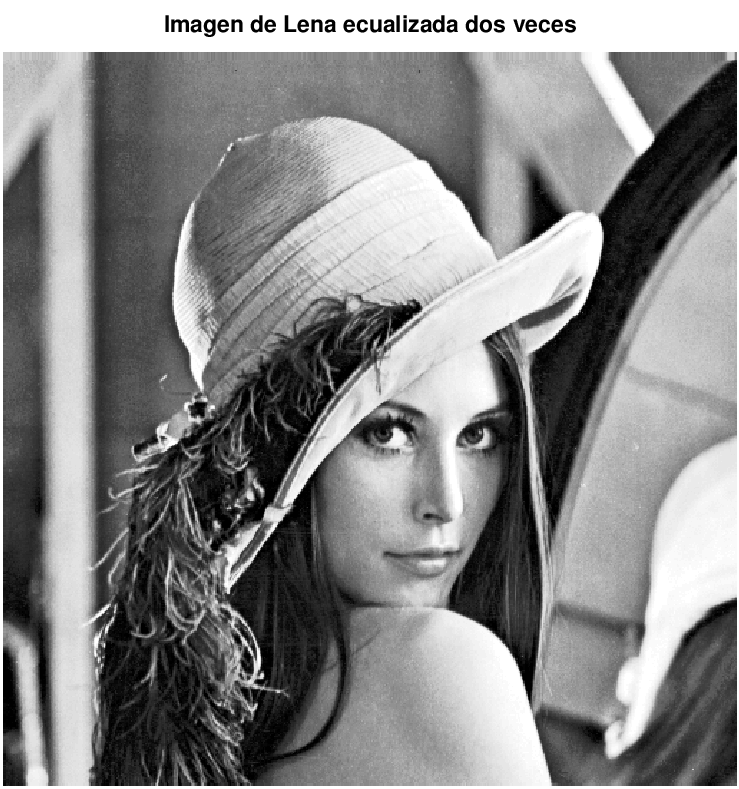
\includegraphics[width=0.9\textwidth]{lenaEqEq.png} % second figure itself
    \subcaption{Imagen de Lena ecualizada 2 veces}
    \end{subfigure}
    \caption{Doble ecualización de imagen de Lena}
\end{figure}

Al aplicar dos veces la ecualización a una misma imagen, se puede observar que el resultado obtenido es prácticamente idéntico. Desde Matlab, se puede observar una leve diferencia entre ambas imágenes al correr el comando \textit{find(...)}. Por ejemplo, en la posición \textit{(49, 49)} de la primer imagen obtenemos el valor 203 mientras que en la segunda obtenemos el valor 204, esto reproduciéndose en los valores que difieren de las imágenes, teniendo variaciones de un entero. Esto puede deberse al manejo de datos no enteros y su redondeamiento. 

La razón por la cual las imágenes obtenidas son idénticas es debido a que la ecualización busca construir una imagen cuyo histograma resultante tenga una distribución uniforme (es decir, distribuir uniformemente los niveles de gris) y, dado que el histograma de una imagen previamente ecualizada ya tiene una distribución uniforme, volver a realizar dicha transformación no genera cambios significantivos. 

\section*{Ejercicio 9}
El archivo correspondiente es \textit{especificacionHistograma.m} y toma como parámetro de entrada una imagen y devuelve la imagen con dicha transformación aplicada.

A continuación presento ejemplos generados al ejecutar la función con la imagen de lena:

\begin{figure}[H]
    \begin{subfigure}{0.5\textwidth}
        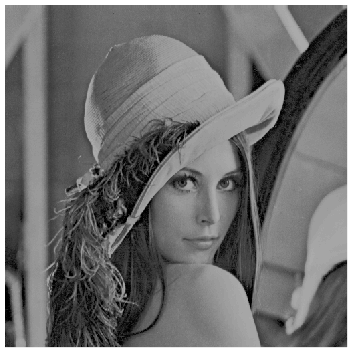
\includegraphics[width=0.9\textwidth]{especLena.png} % first figure itself
    \subcaption{Imagen de Lena generada}
    \end{subfigure}\hfill
    \begin{subfigure}{0.5\textwidth}
        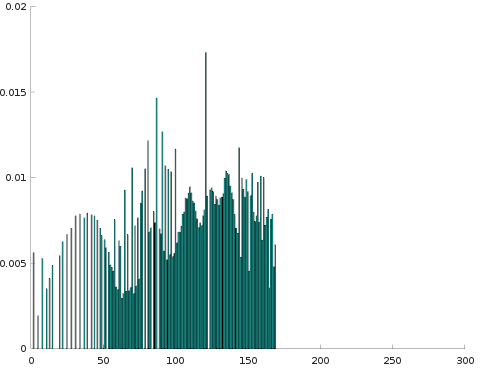
\includegraphics[width=0.9\textwidth]{histoEspecLena.png} % second figure itself
    \subcaption{Histograma generado}
    \end{subfigure}
\end{figure}

\section*{Ejercicio 10}
Para este ejercicio se poseen distintos archivos:
\begin{itemize}
\item \textbf{histogramaModificado.m: }Dada una imagen y un lambda, devuelve la imagen ecualizada generada usando el histograma modificado con lambda y genera una figura mostrando el histograma normalizado, el histograma acumulado y la imagen ecualizada.
\item \textbf{histogramaModificadoSuavizado.m: }Dada una imagen, un lambda y un gamma como parámetros de entrada, devuelve la imagen ecualizada generada usando el histograma modificado con dichos parámetros y genera una figura con el histograma acumulados, una con el histograma nornamlizado y una de la imagen ecualizada.  
\item \textbf{histogramaModificadoSuavizadoVariandoParametros.m: }Dada una imagen, genera múltiples figuras mostrando, en cada una de ellas, para cada valor correspondiente de $\lambda$ y $\gamma$, el histograma normalizado, el histograma acumulado y la imagen ecualizada.
\end{itemize}
Luego de ejecutar la última función con la imagen ``puerta.png", se puede observar cómo el histograma correspondiente a la imagen va teniendo cada vez una distribución más uniforme (generando un función casi lineal en las imágenes de histogramas acumulados) a medida que aumenta el valor de $\lambda$. Además, al ir variando el parámetro de $\gamma$ para un mismo $\lambda$, se puede observar cómo se va suavizando el histograma, es decir que los valores de nivel de gris van aumentando de una manera menos drástica. A continuación se adjuntan gráficos mostrando lo mencionado:
\begin{figure}[H]
    \begin{subfigure}{0.5\textwidth}
        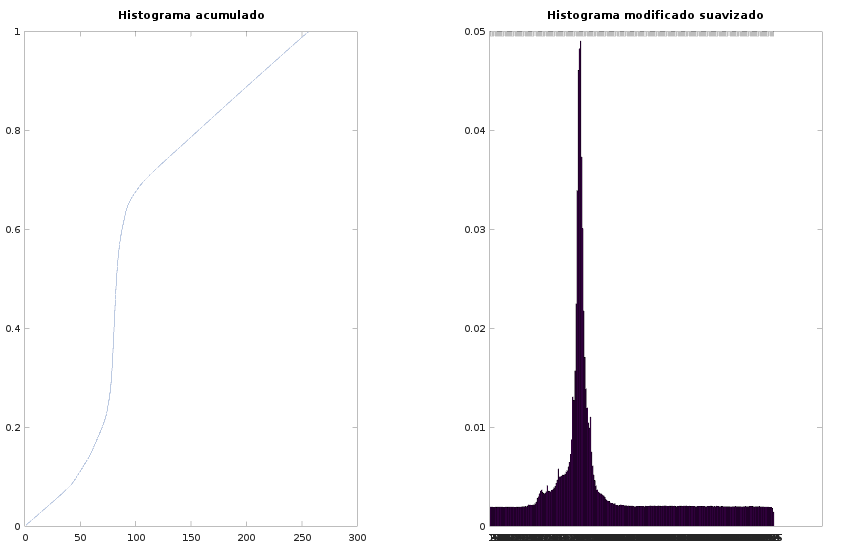
\includegraphics[width=0.9\textwidth]{hpuertita1-1.png} 
    \subcaption{$\lambda=1$, $\gamma=1$}
    \end{subfigure}\hfill
    \begin{subfigure}{0.5\textwidth}
        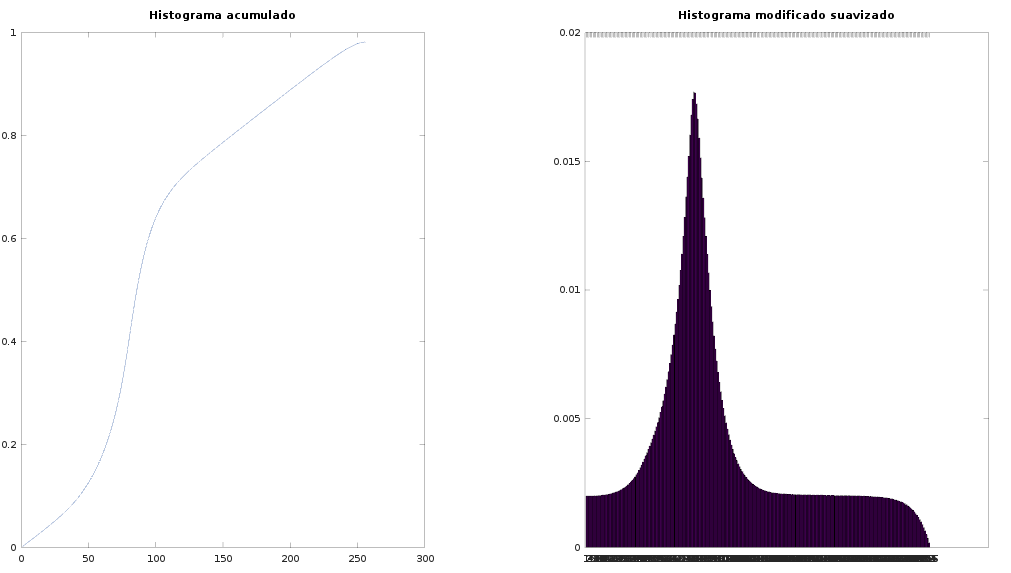
\includegraphics[width=0.9\textwidth]{hpuertita1-200.png} 
    \subcaption{$\lambda=1$, $\gamma=200$}
    \end{subfigure}
\end{figure}

\begin{figure}[H]
    \begin{subfigure}{0.5\textwidth}
        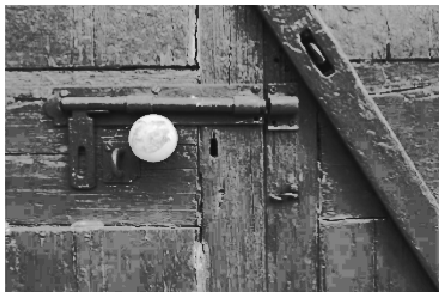
\includegraphics[width=0.9\textwidth]{puertita1-1.png} 
    \subcaption{$\lambda=1$, $\gamma=1$}
    \end{subfigure}\hfill
    \begin{subfigure}{0.5\textwidth}
        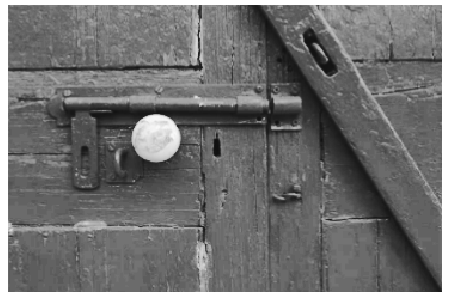
\includegraphics[width=0.9\textwidth]{puertita1-200.png} 
    \subcaption{$\lambda=1$, $\gamma=200$}
    \end{subfigure}
\end{figure}

\begin{figure}[H]
    \begin{subfigure}{0.5\textwidth}
        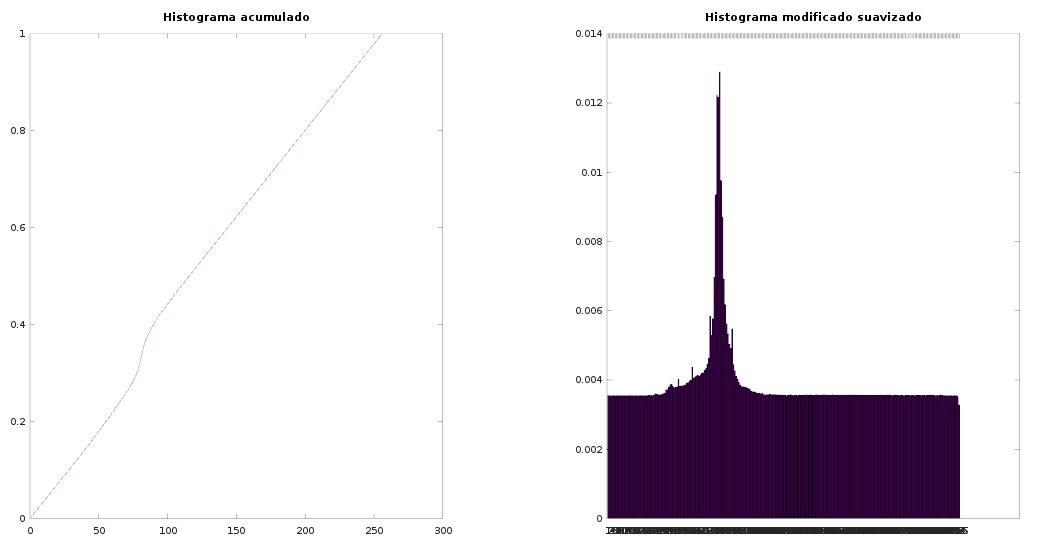
\includegraphics[width=0.9\textwidth]{hpuertita10-1.png} 
    \subcaption{$\lambda=10$, $\gamma=1$}
    \end{subfigure}\hfill
    \begin{subfigure}{0.5\textwidth}
        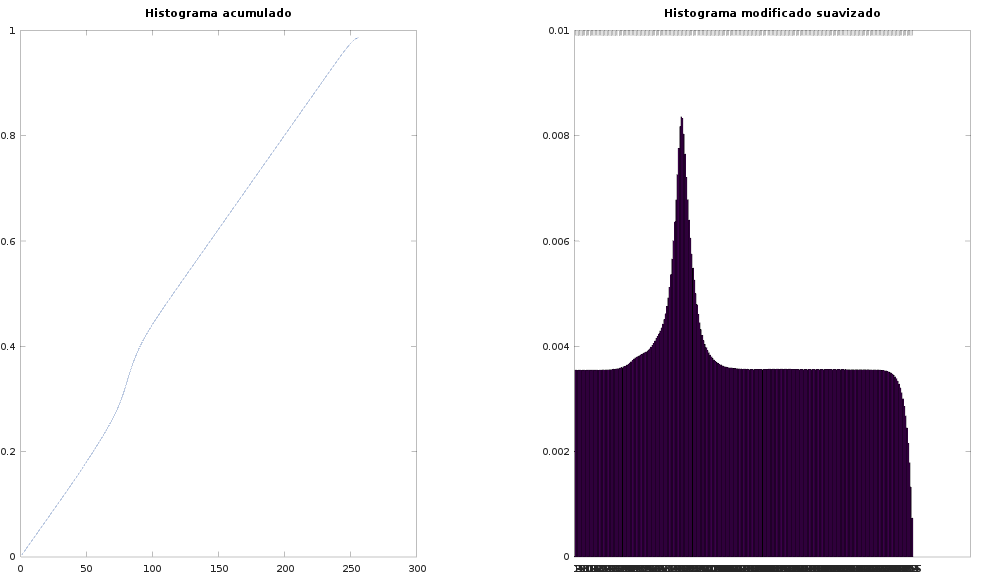
\includegraphics[width=0.9\textwidth]{hpuertita10-200.png} 
    \subcaption{$\lambda=10$, $\gamma=200$}
    \end{subfigure}
\end{figure}

\begin{figure}[H]
    \begin{subfigure}{0.5\textwidth}
        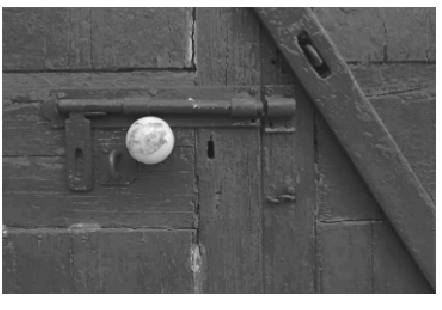
\includegraphics[width=0.9\textwidth]{puertita10-1.png} 
    \subcaption{$\lambda=10$, $\gamma=1$}
    \end{subfigure}\hfill
    \begin{subfigure}{0.5\textwidth}
        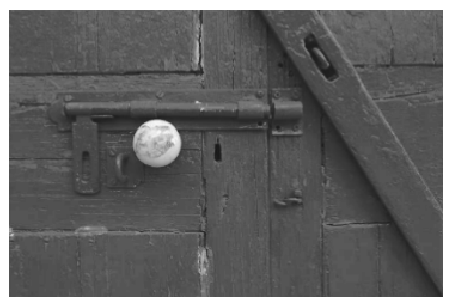
\includegraphics[width=0.9\textwidth]{puertita10-200.png} 
    \subcaption{$\lambda=10$, $\gamma=200$}
    \end{subfigure}
\end{figure}

\begin{figure}[H]
    \begin{subfigure}{0.5\textwidth}
        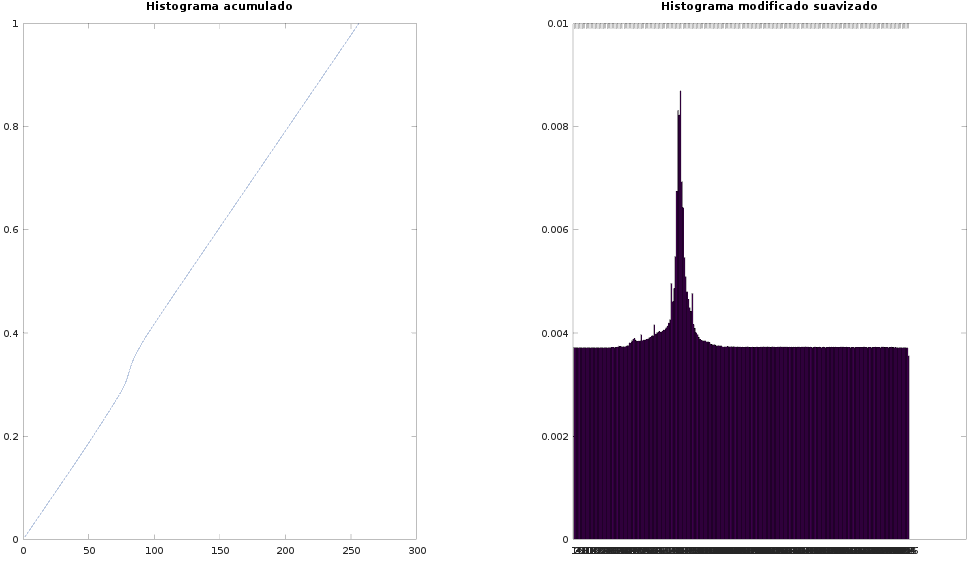
\includegraphics[width=0.9\textwidth]{hpuertita20-1.png} 
    \subcaption{$\lambda=20$, $\gamma=1$}
    \end{subfigure}\hfill
    \begin{subfigure}{0.5\textwidth}
        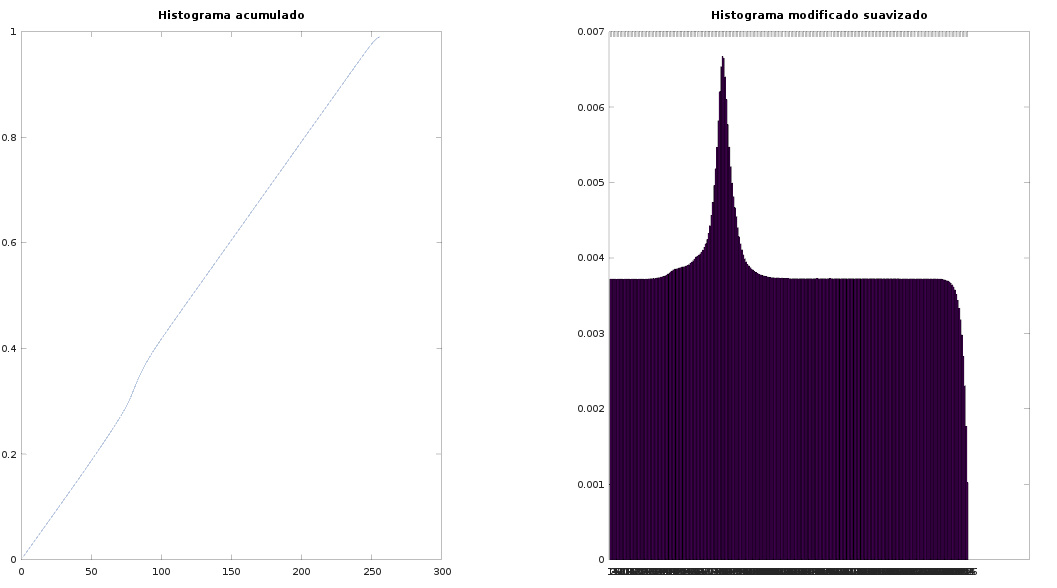
\includegraphics[width=0.9\textwidth]{hpuertita20-200.png} 
    \subcaption{$\lambda=20$, $\gamma=200$}
    \end{subfigure}
\end{figure}

\begin{figure}[H]
    \begin{subfigure}{0.5\textwidth}
        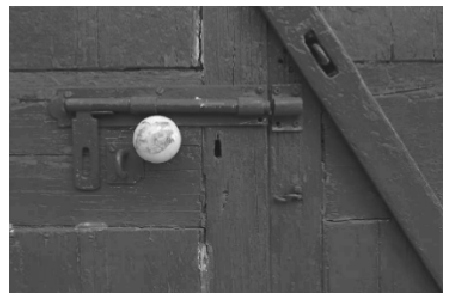
\includegraphics[width=0.9\textwidth]{puertita20-1.png} 
    \subcaption{$\lambda=20$, $\gamma=1$}
    \end{subfigure}\hfill
    \begin{subfigure}{0.5\textwidth}
        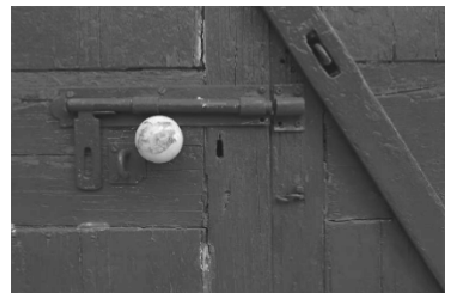
\includegraphics[width=0.9\textwidth]{puertita20-200.png} 
    \subcaption{$\lambda=20$, $\gamma=200$}
    \end{subfigure}
\end{figure}


\end{document}
